\chapter{The Current Thesis}
\label{ch:cur}
\chaptermark{Current Thesis}

% ==========================================================================================================
\newpage

Donec nec arcu lacus, ut dictum purus. Suspendisse tristique turpis vitae enim semper non facilisis ligula posuere. Nulla nulla arcu, pharetra eget bibendum consectetur, eleifend ut tellus. Proin ac tortor erat, quis facilisis leo. Nulla sit amet tellus eu sapien tempus tempor. Vestibulum vehicula lacinia dui non iaculis. 

Pellentesque massa velit, mollis eu lacinia euismod, bibendum sed purus. Duis neque enim, accumsan id euismod ac, pharetra iaculis justo. Cras volutpat, massa id ullamcorper aliquam, ligula dui ultricies libero, id tristique justo magna ac lectus. Suspendisse et aliquet tortor. In non nisl orci, id volutpat odio. 

Maecenas condimentum tincidunt nunc, vitae convallis metus tristique eget. Ut vel mi sed eros sagittis dapibus. Maecenas nibh purus, eleifend vel vulputate in, vehicula at dui. Fusce nec nunc tellus, ac vehicula risus. Aenean semper ligula vitae nisl volutpat tincidunt. Sed id erat vel leo dapibus commodo eget sit amet turpis. Mauris sed eros ac magna egestas volutpat ut a dui. Lorem ipsum dolor sit amet, consectetur adipiscing elit.


\section{Three elements of spontaneous thoughts}
% experience - thought sampling
Integer vulputate vulputate imperdiet. Integer varius elementum urna id hendrerit. Nulla vitae ante leo, id tincidunt purus. Praesent quam lacus, semper vitae tristique pulvinar, gravida sit amet sem. Sed porttitor orci nec orci sodales ac malesuada felis consequat. Aliquam erat volutpat. Cras dapibus dignissim neque non convallis. Ut quis tellus arcu, vitae fermentum orci. Nunc pharetra leo at odio posuere ac pretium odio blandit. Nulla pellentesque tincidunt gravida. 

Phasellus quis metus vel lectus porta vehicula ut eu felis. Mauris libero velit, egestas vel tempus eget, iaculis sit amet magna. Proin accumsan semper consectetur. Nulla et euismod augue. Proin lacus sapien, convallis nec placerat at, vulputate eu massa. Etiam nisi dui, consequat in consequat eget, posuere vel velit. Mauris accumsan venenatis facilisis.

% functional outcome - cognitive measures
Pellentesque massa velit, mollis eu lacinia euismod, bibendum sed purus. Duis neque enim, accumsan id euismod ac, pharetra iaculis justo. Cras volutpat, massa id ullamcorper aliquam, ligula dui ultricies libero, id tristique justo magna ac lectus. Suspendisse et aliquet tortor. In non nisl orci, id volutpat odio. 

Maecenas condimentum tincidunt nunc, vitae convallis metus tristique eget. Ut vel mi sed eros sagittis dapibus. Maecenas nibh purus, eleifend vel vulputate in, vehicula at dui. Fusce nec nunc tellus, ac vehicula risus. Aenean semper ligula vitae nisl volutpat tincidunt. Sed id erat vel leo dapibus commodo eget sit amet turpis. Mauris sed eros ac magna egestas volutpat ut a dui. Lorem ipsum dolor sit amet, consectetur adipiscing elit.

% biological basis - resting state fMRI
Donec nec arcu lacus, ut dictum purus. Suspendisse tristique turpis vitae enim semper non facilisis ligula posuere. Nulla nulla arcu, pharetra eget bibendum consectetur, eleifend ut tellus. Proin ac tortor erat, quis facilisis leo. Nulla sit amet tellus eu sapien tempus tempor. Vestibulum vehicula lacinia dui non iaculis. 

Pellentesque massa velit, mollis eu lacinia euismod, bibendum sed purus. Duis neque enim, accumsan id euismod ac, pharetra iaculis justo. Cras volutpat, massa id ullamcorper aliquam, ligula dui ultricies libero, id tristique justo magna ac lectus. Suspendisse et aliquet tortor. In non nisl orci, id volutpat odio. 

Aliquam imperdiet est id nulla fringilla vel luctus tellus pretium. Aliquam tincidunt ante nec lacus ullamcorper placerat. In bibendum, turpis vitae dapibus interdum, elit quam tempus nisi, ac vestibulum nulla nisl vel mauris. Nullam ut diam nisi. Vestibulum vitae eros sed felis fermentum ultrices. Integer tincidunt, justo vel luctus gravida, leo erat placerat ipsum, sit amet condimentum diam massa ac ligula. 

Etiam nec ullamcorper lectus. Quisque auctor libero facilisis risus volutpat vitae auctor felis fermentum. Mauris non sapien eget metus laoreet lacinia eget ac magna. Sed sed leo leo. Curabitur in est at quam condimentum semper sit amet sed ipsum. Nam neque est, auctor posuere varius ac, bibendum sit amet urna. 

Nunc lobortis tortor id orci molestie pulvinar suscipit ipsum mattis. Maecenas auctor mi mauris. Nunc condimentum lectus eu libero ornare commodo. Mauris cursus felis quis nunc ornare a blandit sem commodo. Vestibulum eu neque ut est hendrerit condimentum. Ut nisl mi, tristique ut malesuada aliquet, imperdiet a quam. Nam malesuada accumsan massa, sit amet ullamcorper ante mattis at.

\begin{figure}[H]
	\centering
	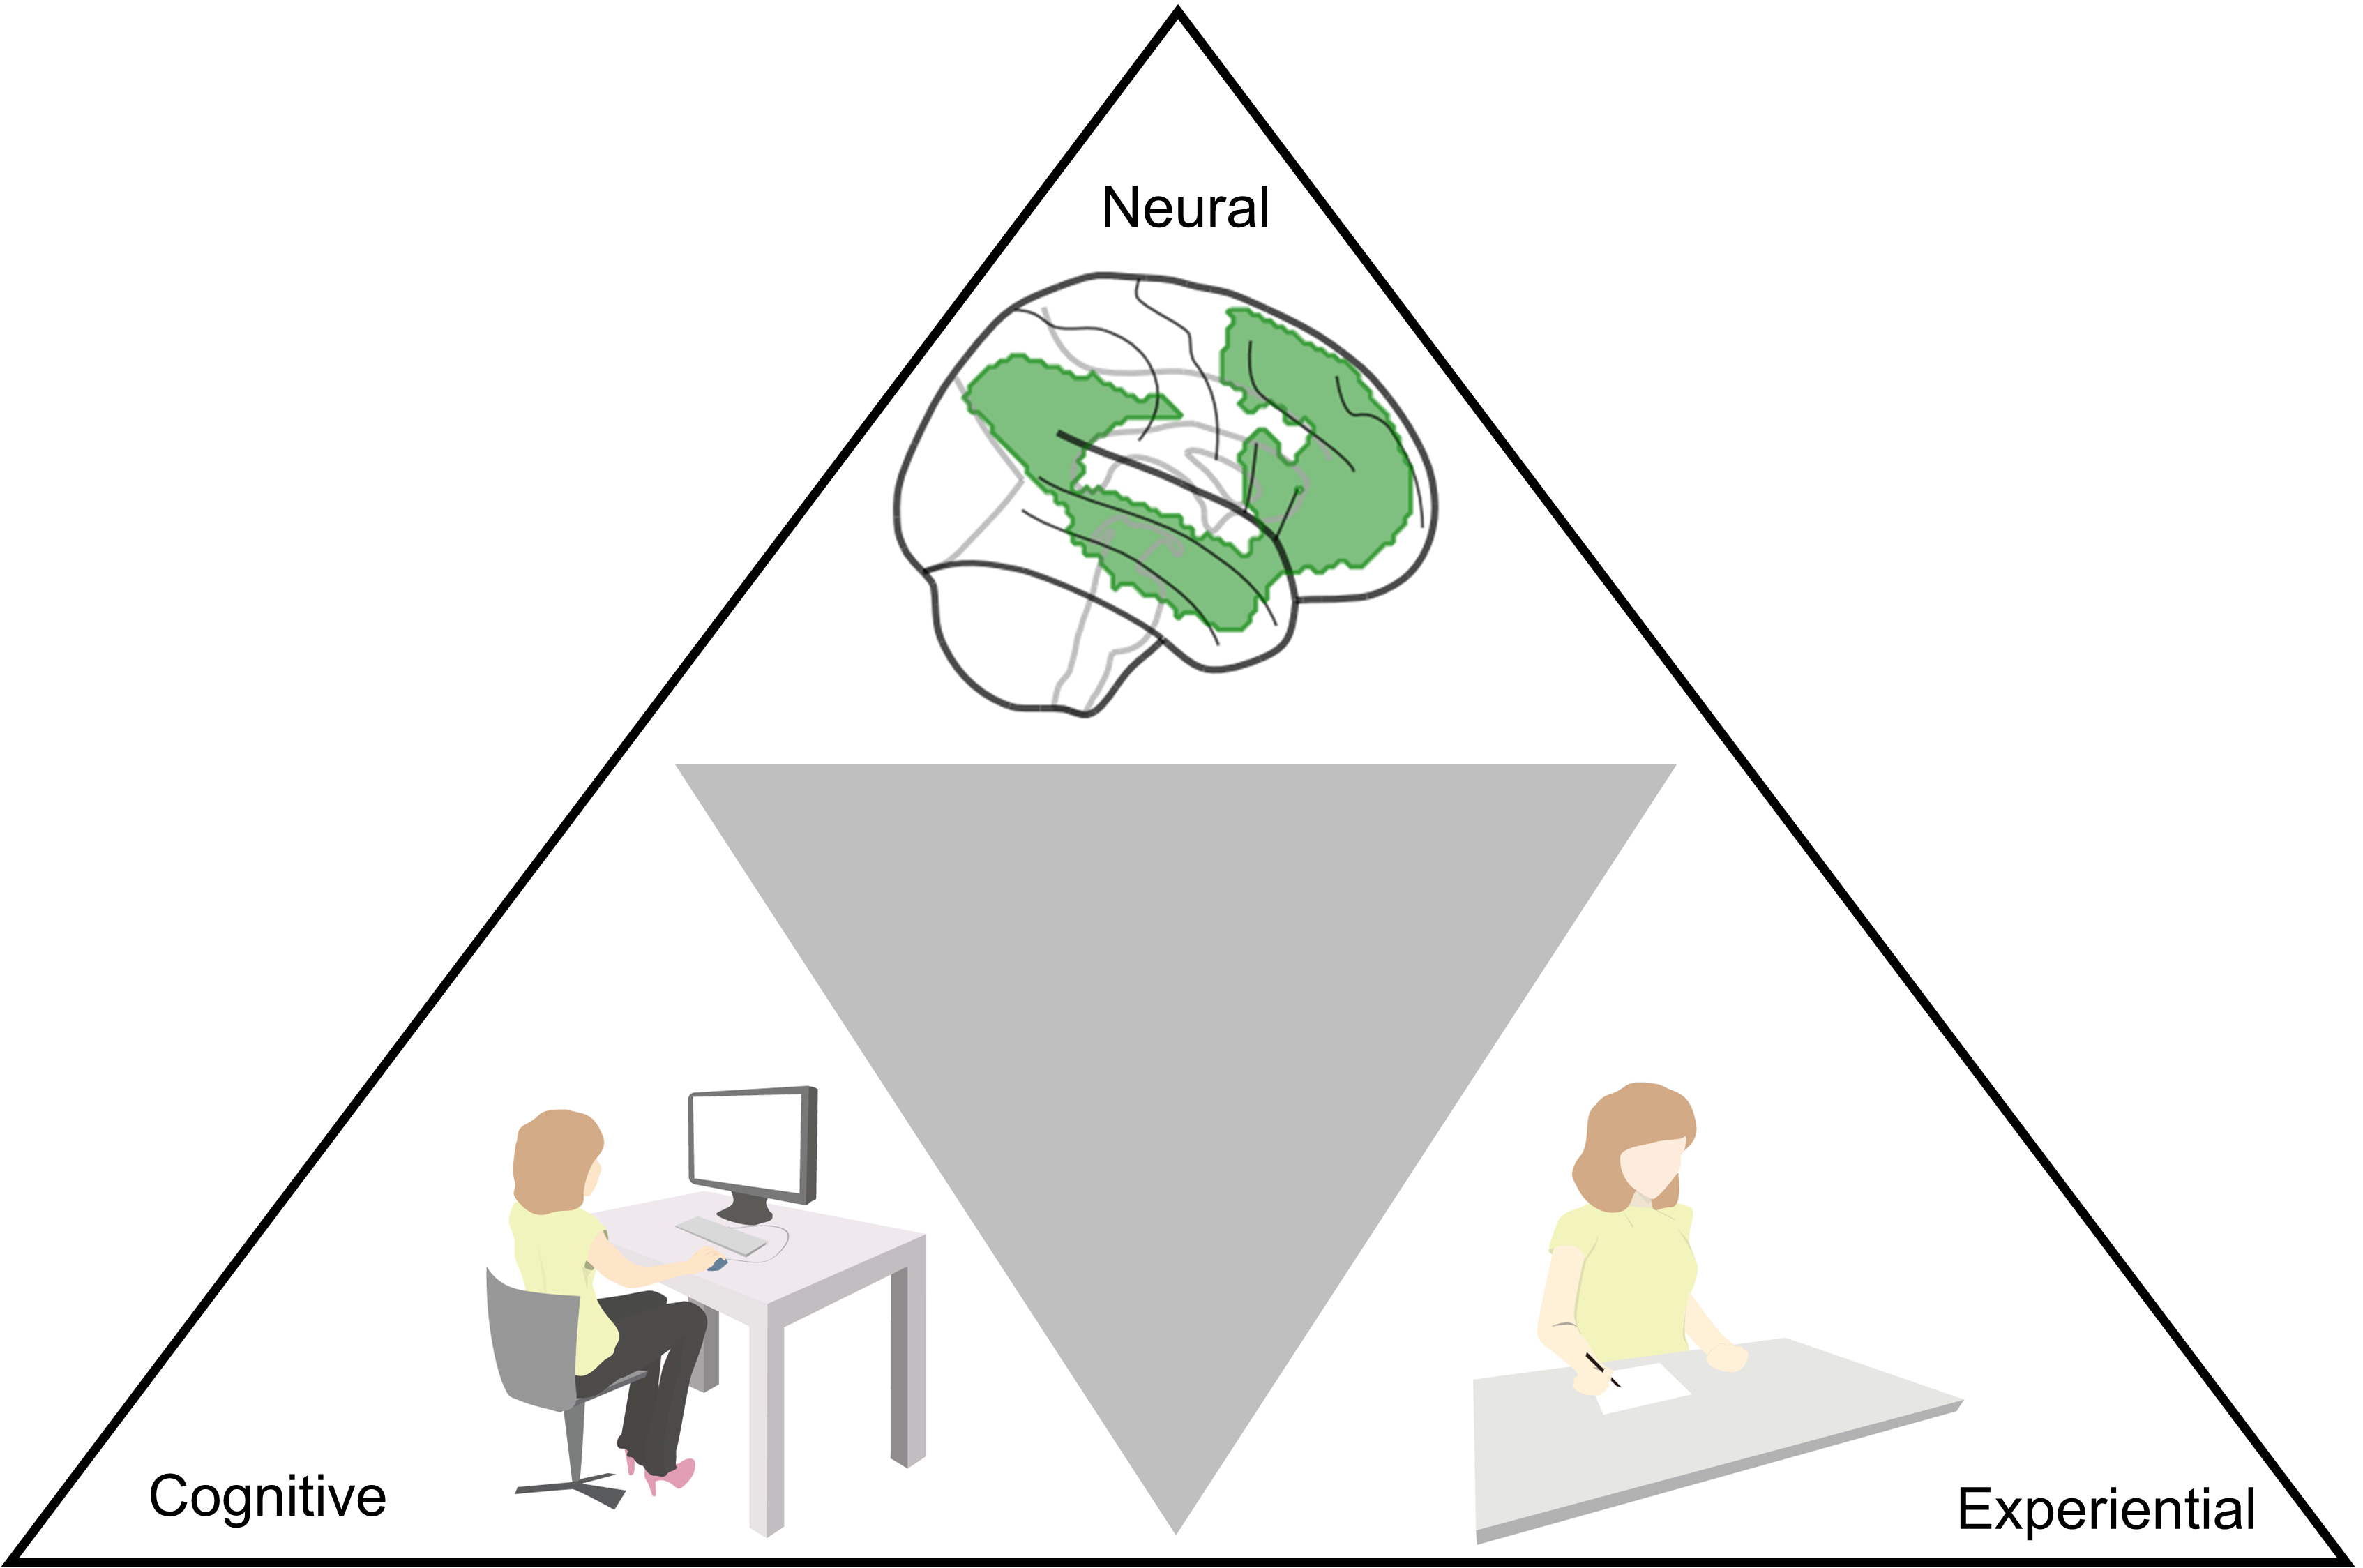
\includegraphics[width=0.8\textwidth]{chapters/img/thesisfig1.png}
	\caption{Schematic of the thesis} 
	\label{fig:thesis:fig1}
\end{figure}

\section{Sparse canonical correlation analysis}

% the method
Integer vulputate vulputate imperdiet. Integer varius elementum urna id hendrerit. Nulla vitae ante leo, id tincidunt purus. Praesent quam lacus, semper vitae tristique pulvinar, gravida sit amet sem. Sed porttitor orci nec orci sodales ac malesuada felis consequat. Aliquam erat volutpat. Cras dapibus dignissim neque non convallis. Ut quis tellus arcu, vitae fermentum orci. Nunc pharetra leo at odio posuere ac pretium odio blandit. Nulla pellentesque tincidunt gravida. 

Phasellus quis metus vel lectus porta vehicula ut eu felis. Mauris libero velit, egestas vel tempus eget, iaculis sit amet magna. Proin accumsan semper consectetur. Nulla et euismod augue. Proin lacus sapien, convallis nec placerat at, vulputate eu massa. Etiam nisi dui, consequat in consequat eget, posuere vel velit. Mauris accumsan venenatis facilisis.

% why sparse
Integer vulputate vulputate imperdiet. Integer varius elementum urna id hendrerit. Nulla vitae ante leo, id tincidunt purus. Praesent quam lacus, semper vitae tristique pulvinar, gravida sit amet sem. Sed porttitor orci nec orci sodales ac malesuada felis consequat. Aliquam erat volutpat. Cras dapibus dignissim neque non convallis. Ut quis tellus arcu, vitae fermentum orci. Nunc pharetra leo at odio posuere ac pretium odio blandit. Nulla pellentesque tincidunt gravida. 

Phasellus quis metus vel lectus porta vehicula ut eu felis. Mauris libero velit, egestas vel tempus eget, iaculis sit amet magna. Proin accumsan semper consectetur. Nulla et euismod augue. Proin lacus sapien, convallis nec placerat at, vulputate eu massa. Etiam nisi dui, consequat in consequat eget, posuere vel velit. Mauris accumsan venenatis facilisis.

% why CCA is good for this thesis
Integer vulputate vulputate imperdiet. Integer varius elementum urna id hendrerit. Nulla vitae ante leo, id tincidunt purus. Praesent quam lacus, semper vitae tristique pulvinar, gravida sit amet sem. Sed porttitor orci nec orci sodales ac malesuada felis consequat. Aliquam erat volutpat. Cras dapibus dignissim neque non convallis. Ut quis tellus arcu, vitae fermentum orci. Nunc pharetra leo at odio posuere ac pretium odio blandit. Nulla pellentesque tincidunt gravida. 

Phasellus quis metus vel lectus porta vehicula ut eu felis. Mauris libero velit, egestas vel tempus eget, iaculis sit amet magna. Proin accumsan semper consectetur. Nulla et euismod augue. Proin lacus sapien, convallis nec placerat at, vulputate eu massa. Etiam nisi dui, consequat in consequat eget, posuere vel velit. Mauris accumsan venenatis facilisis.

\section{Summary}

In the current PhD, we would like to explore the numerous thoughts to describe human consciousness experience and establish a framework that incorporate the heterogeneity of the mind-wandering experience. The wide range of functional outcomes and contents of the mind-wandering state is perplexing as often time, those features are contradictory against each other. These studies indicated that the mind-wandering state is a heterogeneous collection of experiences that each type of the mind-wandering experiences has its own underlying cognitive mechanism and contextual representation (Smallwood \& Andrews-Hanna, 2013). The current difficulty of advancing the mind-wandering research is that, although the related cognitive and experience phenotypes has been found, we are unsure about the mechanism uniting those features. Moreover, the integrative nature of higher level cognition makes it difficult to identify the contribution of different processes to the mind-wandering state. This PhD aims to advance the understanding of the identified cognitive processes and find the quantifiable features of the cognitive measures that can infer the mind-wandering states. With the combination of MDES that accesses the heterogeneity of the content, cognitive phenotypes and the neuroimaging data, this PhD aims to establish the ontology of spontaneous thoughts and lays a solid foundation for future studies in consciousness. 
